%!TEX root = ../dokumentation.tex

\chapter{Medizinische Grundlagen}

\section{Herzparameter}
Das menschliche Herz kann mit vielen verschiedenen Werten parametrisiert werden. Der wohl bekannteste Parameter ist dabei die Herzfrequenz (Hf). Sie gibt an, wie oft das Herz in einer bestimmten Zeit schlägt. Meist wird dafür das Zeitintervall einer Minute gewählt und die in dieser Zeit gemessenen Herzschläge in der Einheit \emph{bpm} (beats per minute) angegeben. 
\subsection{Herzfrequenz (Hf)} \label {subsec:hf}
Die Herzfrequenz ist abhängig von verschiedenen Faktoren. So spielen beispielsweise Alter und körperliche Fitness eine große Rolle. Bei trainierten (Ausdauer) Sportlern schlägt das Herz in Ruhe bedeutend seltener als bei untrainierten Personen. Dies kann damit erklärt werden, dass durch das Ausdauertraining das \textbf{Schlagvolumen (SV)} erhöht werden kann. Das Schlagvolumen gibt an, wie viel Blut das Herz mit einem Schlag durch den Körper pumpen kann. Wenn sich dieses Volumen also erhöht, muss das Herz seltener schlagen, um das \textbf{Herzminutenvolumen (HMV)} zu halten. Dieses berechnet sich aus Herzfrequenz und Schlagvolumen. \cite{herz} 
\begin{equation}\formelentry{Herzminutenvolumen (HMV)}
	%Herzminutenvolumen = Herzfrequenz * Schlagvolumen
	HMV = Hf * SV
\end{equation} 
Bei körperlicher Belastung, beispielsweise sportlicher Aktivität, erhöht sich das benötigte Herzminutenvolumen, da die Muskeln mehr Sauerstoff brauchen. Da sich das Schlagvolumen des Herzens nicht anpassen lässt, erhöht sich die Herzfrequenz, um dem benötigten Herzminutenvolumen gerecht zu werden. Grundsätzlich, wie jeder bei sich selber feststellen kann, erhöht sich die Herzfrequenz bei körperlicher Aktivität. Durch sehr starker Aktivität kann die Herzfrequenz auf ein Maximum ansteigen. Die maximale Herzfrequenz kann mit folgender Faustformel abgeschätzt werden: 
\begin{equation}\formelentry{Maximale Herzfrequenz}
	%maximale Herzfrequenz = 220 - Alter
	Hf_{max} = 220 - Alter
\end{equation}
Bei diesem Wert wird häufig auch vom Maximalpuls gesprochen. Allerdings muss zwischen Puls und Herzfrequenz unterschieden werden, da diese nicht identisch sind. 
Die Herzfrequenz beschreibt, wie bereits in den vorhergehenden Abschnitten beschrieben, die tatsächlichen Schläge des Herzens. Zur Messung der Herzfrequenz kann ein EKG genutzt werden,
Der \textbf{Puls} hingegen wird peripher, beispielsweise am Hals oder Handgelenk gemessen. Dabei werden Pulswellen erfasst, welche sich durch den Körper bewegen. Eine Pulswelle entsteht, wenn das Herz schlägt, und das Blut durch den Körper pumpt. Dabei wird das Blut gegen die Arterienwände gedrückt und eine Pulswelle kann detektiert werden.
Bei gesunden Menschen entspricht der Puls der Herzfrequenz, da jeder Herzschlag Blut durch den Körper pumpt und somit auch eine messbare Pulswelle erzeugt. Bestimmte Herzrhythmuskrankheiten können dafür verantwortlich sein, dass Puls und Herzfrequenz voneinander abweichen. Dabei können Kontraktionen des Herzens entstehen, welche kein oder nicht genug Blut durch den Körper pumpen, um eine messbare Pulswelle zu erzeugen. Die Differenz zwischen Herzfrequenz und Puls nennt sich \textbf{Pulsdefizit} (und ist bei gesunden Menschen 0). \cite{babilon}

Die Variation der Herzfrequenz wird über das \textbf{vegetative Nervensystem} geregelt. Dies besteht aus dem \textit{Sympathikus} und seinem Gegenspieler, dem \textit{Parasympathikus}. Außerdem ist das \textit{enterische Nervensystem (Eingeweidenervensystem)} teil des vegetativen Nervensystems. Dies spielt für die Steuerung des Herzens allerdings keine Rolle und wird daher im Laufe dieser Arbeit nicht mehr erwähnt. Ebenso haben Sympathikus und Parasympathikus Funktionen in der Verdauung. Da dies ebenfalls keine Relevanz für das Herz hat, wird darauf nicht weiter eingegangen. Die folgende Erklärung von Sympathikus und Parasympathikus beziehen sich daher nur auf die für das Herz relevanten Eigenschaften.\cite{veg}

\begin{enumerate}
	\item \textbf{Sympathikus} 
	
	Der Sympathikus kann den Organismus auf eine Aktivitätssteigerung ("fight or flight") einstellen. Er ist der dominante Teil des vegetativen Nervensystems, wenn es um Stresssituationen geht. Wenn diese eintritt, wird die Aktivität von situationsbedingt unwichtigen Organen, beispielsweise Darm oder andere Organe, die zur Verdauung beitragen, gesenkt. 
	Die Aktivität von Organen, die in Stresssituationen wichtig sind, wird verstärkt. So werden beispielsweise die Pupillen vergrößert.
Die Herzfrequenz wird stark erhöht.\cite{sym}	
	
	\item \textbf{Parasympathikus}
	
	Der Parasympathikus stellt den Organismus auf Ruhesituationen ("rest and digest") ein. So werden in den dominanten Phasen des Parasympathikus Organe mit Verdauungsfunktionen in ihrer Aktivität gestärkt. Der Körper wird auf Entspannung und Regeneration heruntergefahren. 
	Die Herzfrequenz wird in diesen Phasen gesenkt.\cite{para}
\end{enumerate}

Das vegetative Nervensystem ist in seiner Funktion \textbf{unwillkürlich}. Das bedeutet, es kann nicht bewusst von der jeweiligen Person gesteuert werden. Dadurch sind Messungen, beispielsweise an der Herzfrequenz sehr gut geeignet, um bestimmte äußere Einflüsse zu untersuchen.
Die Ergebnisse können nicht von der Testperson verfälscht werden, da sie das vegetative Nervensystem nicht beeinflussen kann. (Andere äußere Einflüsse wie Aufregung müssen berücksichtigt werden und können das Ergebnis logischerweise verfälschen.)\cite{veg}
		
Um nun den konkreten Einfluss von elektromagnetischen Wellen zu untersuchen, kann die Herzfrequenz als Messparameter benutzt werden. Ein weiterer Parameter, welcher stark abhängig vom vegetativen Nervensystem ist, ist die \textbf{Herzfrequenzvariabilität (HRV)}. Im Verlauf dieser Arbeit, wird die Herzratenvariabilität als entscheidender Parameter genutzt. Alle durchgeführten Messungen und daraus abgeleiteten Interpretationen beziehen sich auf diese. 


\section{Herzfrequenzvariabilität (HRV)}
Die Herzfrequenzvariabilität, auch Herzratenvariabilität, ist die zeitliche Variation zwischen zwei Herzschlägen. Sie ist einer der wichtigsten Parameter des menschlichen Herzens. Ein gesunder Mensch hat keinen vollständig gleichmäßigen Herzschlag. Für Personen, die sich nicht mit der HRV auskennen, hört sich dies erst einmal verwunderlich an. Im Folgenden soll jedoch die HRV und deren Bedeutung erläutert werden. \\
Um die HRV besser erklären zu können, wird folgendes Beispielszenario verwendet: Das Herz eines Menschen schlägt 60 Mal pro Minute. Die Person ruht währenddessen vollständig, sodass von einem konstanten Puls von 60 ausgegangen wird. Nun stellt sich die Frage nach der Zeit zwischen den einzelnen Herzschlägen. Auf den ersten Blick liegt es nahe davon auszugehen, dass zwischen jedem Herzschlag die gleiche Zeit, also eine Sekunde vergeht. Dies ist jedoch nicht richtig. Die Zeit zwischen den einzelnen Schlägen des Herzens, die HRV,  variiert deutlich.  Bei einem gesunden Menschen beträgt der Wert der HRV ungefähr 100ms. Am gezeigten Beispiel ist dies eine Abweichung von bis zu 10 \%.\cite[S.20ff]{babilon}\cite{hrv} \\

Mithilfe dieser Abweichungen lassen sich Aussagen über den Gesundheitszustand des Menschen treffen. Dabei spielt das bereits erklärte vegetative Nervensystem eine wichtige Rolle. Ein gutes Zusammenspiel zwischen Sympathikus und Parasympathikus sind Teil eines gesunden Menschen. Mithilfe der HRV kann dieses Zusammenspiel gut messbar und "in Zahlen ausgedrückt werden". 
Grundsätzlich lässt sich sagen, dass eine hohe HRV ein Zeichen für einen gesunden Organismus ist. So können zum Beispiel eine ausgewogene Ernährung oder ausreichend Schlaf zu einer Erhöhung der Herzfrequenzvariabilität führen. Im Gegensatz dazu wirken sich Stress, gesundheitsschädliche Medikamente oder Schlafmangel negativ auf die HRV aus.\cite{hrv} \\
Auch im Bereich des Sports spielt die HRV eine wichtige Rolle, da sie eine große Aussagekraft über die Regeneration des Athleten hat. Es gibt Trainingspläne, in welchen nach dem Wert der HRV trainiert wird. So wurde bereits 2007 ein Artikel veröffentlicht \cite{sport}, welcher das Training mit Beachtung der HRV beschreibt. In diesem Artikel wurde das Ausdauertraining von 26 Männern untersucht. Diese wurden dabei in drei Gruppen aufgeteilt. Eine Gruppe trainierte dabei einen festgelegten Trainingsplan von sechs Einheiten (4 Hochintensitätstraining, 2 Trainings mit niederer Intensität) .\\
Die zweite Gruppe trainierte individuell nach dem Wert ihrer HRV. War die Herzfrequenzvariabilität bei der Messung am Morgen hoch, so wurde mit hoher Intensität trainiert. Bei einer niederen HRV wurde nur mit niederer Intensität oder gar nicht trainiert. Die dritte Trainingsgruppe war eine Kontrollgruppe. 
Am Ende des vierwöchigen Trainingsprogramms konnte bei der individuell nach HRV Wert trainierenden Trainingsgruppe eine stärkere Verbesserung der Ausdauer (Untersuchung verschiedener Parameter, welche Aussagen über die Ausdauer zulassen (Beispiel: VO2max)) im Vergleich zur Gruppe mit festem Trainingsplan festgestellt werden.\cite{sport}\\

Die Wichtigkeit der HRV wurde nun bereits deutlich. Wie diese gemessen wird und welche Aussagekraft die verschiedenen Parameter der HRV haben, soll nun genauer erläutert werden.

\subsection{Messung}
In der folgenden Grafik ist eine EKG Messung eines menschlichen Herzens zu sehen.
\begin{figure}[H]
    \centering
    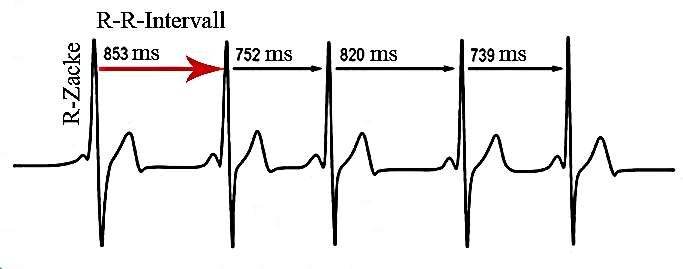
\includegraphics[width=0.7\linewidth]{RR}
    \caption{R-R-Intervall}
    \label{fig:R-R-Intervall}
    \cite{rrbild}
\end{figure}

 Gut erkennbar sind dabei die hohen R Zacken. Diese werden benutzt, um die Herzfrequenzvariabilität zu berechnen.
 Für die Berechnung wird die Zeit zwischen zwei aufeinanderfolgenden R Zacken benötigt. Diese Zeitspanne wird als R(-)R-Intervall bezeichnet. Mit diesem Begriff muss jedoch vorsichtig umgegangen werden, da er leicht verwechselt wird. Beim Messen des Blutdrucks wird ebenfalls die Abkürzung RR verwendet. In diesem Zusammenhang ist jedoch von der Blutdruckmessmethode nach \textit{Riva-Rocci} die Rede. Um eine Verwechslung zu vermeiden, wird das R(-)R-Intervall der HRV in der Literatur häufig als NN-Intervall bezeichnet. Dieser unterscheidet sich inhaltlich jedoch leicht vom Begriff des RR-Intervalls. 
 Das RR-Intervall ist die Zeit zwischen allen R-Zacken der Messung. Während einer Messung können Störungen auftreten, welche zusätzliche "Zacken" verursachen. Diese verfälschen die Messung und nennen sich \textit{Artefakte}\cite{artefakt}. Im RR-Intervall werden diese trotzdem berücksichtigt.\\
 Das NN-Intervall ist die Zeit zwischen den \textit{normalen} R-Zacken. Hier werden die fälschlich gemessenen R-Zacken nicht berücksichtigt und herausgefiltert. Trotz dieses eigentlichen inhaltlichen Unterschieds zwischen den Begriffen RR- und NN-Intervall werden diese oft als Synonym füreinander verwendet. So auch in dieser Ausarbeitung.\cite{rr}\cite{kubios}
 

 Im Gegensatz zur Herzfrequenz gibt es bei der HRV nicht nur einen Wert. Die Herzfrequenzvariabilität besitzt viele Parameter, welche alle unterschiedlich berechnet werden. Bevor die Berechnung der verschiedenen Parameter erklärt wird, muss zuerst verstanden werden, weshalb es überhaupt so viele Parameter gibt und was diese aussagen.
 
 \subsection{Nutzen}
 Mit den verschiedenen Parametern lassen sich grundsätzliche Feststellungen über den Gesundheitszustand treffen. Besonders für Aussagen über das vegetativen Nervensystem ist die HRV sehr geeignet. Da die Unterschiede der Parameter der HRV noch nicht genau erklärt wurde, ist im Folgenden mit dem Begriff HRV immer die Gesamtheit aller Parameter gemeint. Messungen der HRV sind gut dafür geeignet, um Aussagen über die Erholungsfähigkeit zu treffen. Da auch psychische Belastungen Auswirkungen auf die HRV haben, kann sie für auch als Grundlage für grundsätzlichen Gesundheitszustand und Fitness genutzt werden. \\
Grundsätzlich lässt sich sagen, dass die HRV aufgrund ihrer starken Abhängigkeit vom vegetativen Nervensystem und großer Aussagekraft über den menschlichen Körper sehr gut für Messungen der Aktivität des vegetativen Nervensystem geeignet ist. 
 

 \subsection{Parameter}
 
 Die HRV kann mit vielen verschiedenen Parametern dargestellt werden, welche sich alle in die folgenden 3 Gruppen aufteilen lassen:
 
 \begin{enumerate}
 	\item Zeitabhängige Parameter
 	\item Frequenzabhängige Parameter
 	\item Nicht-lineare Parameter
\end{enumerate}

Diese drei Gruppen sollen nun anhand von Beispielen genauer betrachtet werden. Dabei soll grundsätzlicher Aufbau der Analyse als auch die Nutzung der jeweiligen Parameter beschrieben werden.

\subsubsection{Zeitabhängige Parameter}	
Zeitabhängige Parameter sind mathematisch am einfachsten zu greifen, da keine mathematischen Operationen auf die Messwerte angewendet werden. Es werden einfache Rechnungen mit den Messungen durchgeführt. Wichtige Parameter für Zeitabhängige Parameter sind:   
 
 \begin{figure}[H]
 	\centering
 	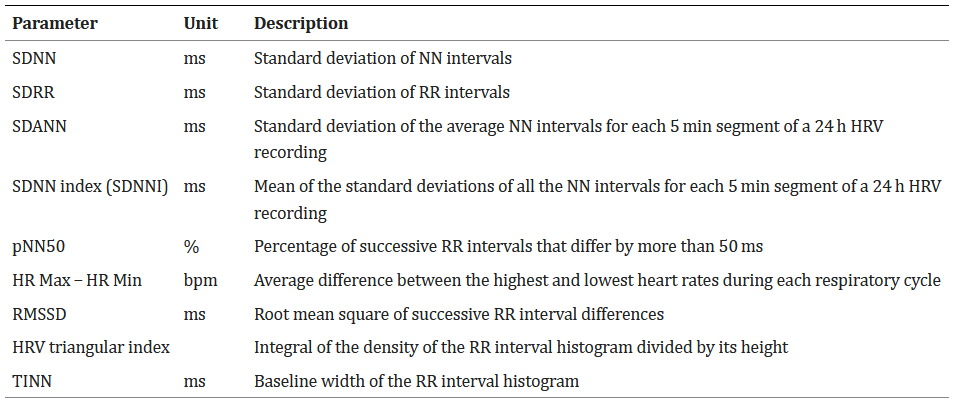
\includegraphics[width=1.0\linewidth]{HRVfreq}
 	\caption{HRV - Zeitabhängige Parameter}
 	\label{fig:HRVfreq}
 	\cite[S.2]{med}
 \end{figure}
Alle dargestellten Parameter zu erklären würde den Umfang der Arbeit übersteigen, sodass nur einige ausgewählte Parameter in ihrer Berechnung erläutert werden. Bei weiterem Interesse an den anderen Parametern können genauer Informationen unter \cite{med} nachgelesen werden. 

\paragraph{SDNN (Standard Deviation of NN-Intervals)}\mbox{} \\
Der SDNN beschreibt die Standard-Abweichung der NN-Intervalle und wird in der Einheit ms angegeben. Er zeigt, wie stark die einzelnen Werte vom Durchschnitt abweichen. Mit folgender Formel kann der SDNN berechnet werden: 
\begin{equation}\formelentry{SDNN}
	%SDNN
SDNN = \sqrt{\dfrac{1}{N-1} * \sum\limits_{i=1}^{N}  (RR_i - \overline{RR})^{2}}
\end{equation}
Wenn der SDNN einen beispielhaften Wert von 40 ms beträgt, ist die Zeit zum nächsten Herzschlag 40 ms länger oder kürzer als die Zeit zum vorhergehenden Herzschlag. Grundsätzlich lässt sich sagen, je höher der SDNN, desto besser.\\

Der SDNN wird häufig genutzt, um eine Aussage über die Gesamtheit des autonomen Nervensystems zu treffen, weswegen er weder Sympathikus noch Parasympathikus zugeordnet ist.\cite[S.22]{babilon}  Über die Dauer einer Messung nimmt der SDNN stetig zu. Daher ist es äußert wichtig, dass, wenn Werte des SDNN verglichen werden, Messungen mit gleicher Länge als Berechnungsgrundlage vorliegen. Auch sollten die äußeren Umstände so ähnlich wie möglich sein.\cite{zeit}\\
SDNN Werte, welcher einer Messung über 24 Stunden entspringen, werden häufig genutzt, um Patienten mit Herzkrankheiten zu untersuchen und einzuteilen. So werden Patienten mit einem SDNN unter 50 ms als nicht gesund eingestuft. Bei einem Wert zwischen 50 und 100 ms wird die Gesundheit als beeinträchtigt angesehen und ab einem Wert von über 100 ms gilt der Patient als gesund. \cite[S.4]{med}  

\paragraph{RMSSD (Root Mean Square of successive differences)}\mbox{} \\
Wenn in Pulsuhren, Apps oder Artikeln nur von der HRV die Rede ist, jedoch kein genauer Parameter spezifiziert wird, ist mit einer hohen Wahrscheinlichkeit der RMSSD gemeint. Er ist nämlich einer der bekanntesten Parameter der HRV und wird dazu benutzt, um Aussagen über die (kurzzeitige) Erholungsfähigkeit des Körpers auszusagen. Erholung ist für einen Menschen essenziell und daher auch Indikator für einen gesunden Organismus. Deshalb können mithilfe Messungen der Erholungsfähigkeit, den RMSSD, Aussagen über grundsätzlichen Gesundheitszustand und Fitness abgeleitet werden.
Ein hoher RMSSD Wert zeigt dabei, dass der Körper sich gut erholen kann. Auch lassen sich positive Schlüsse auf den Umgang mit (psychischem) Stress ziehen. 
Auf der anderen Seite deutet ein niederer RMSSD Wert eine weniger gute Erholungsfähigkeit des Körpers an. Ursachen können dabei physische oder psychische Anstrengung sein. Auch kann ein niedriger RMSSD Wert ein Indiz für Krankheiten sein.\\
 Die Studie \cite{sudep} untersucht beispielsweise den Zusammenhang zwischen RMSSD und SUDEP(sudden unexpected death in epilepsy, deutsch: plötzlich und unerwarteter Todesfall bei Epilepsie). Dabei wird festgestellt, dass das SUDEP-Risiko bei Epilepsiepatienten mit niederen RMSSD Werten höher ausfällt. Der RMSSD und grundsätzlich die HRV stehen also in direktem Zusammenhang zum SUDEP-Risiko. 

Aufgrund der großen Aussagekraft über die Erholungsfähigkeit im Körper kann der RMSSD im autonomen Nervensystem klar dem Parasympathikus zugeordnet werden und unterscheidet sich hiermit klar vom SDNN.\cite[S.22]{babilon}

Die Berechnung des RMSSD sieht wie folgt aus:
\begin{equation}\formelentry{RMSSD}
	%RMSSD
	RMSSD = \sqrt{\dfrac{1}{N-1} * \sum\limits_{i=1}^{N}  (RR_{i+1} - RR_i)^{2}}
\end{equation}
In der Berechnung werden die einzelnen aufeinanderfolgenden NN-Intervalle quadratisch addiert. Danach wird dies durch die Anzahl der NN-Intervalle geteilt. Abschließend wird die Wurzel gezogen, um die durchschnittliche Abweichung zwischen aufeinanderfolgende Intervalle zu erhalten. Angegeben wird der RMSSD in Millisekunden.\cite{rmssdart}\cite{zeit} \\


\paragraph{pNN50}\mbox{} \\
Ein weiterer wichtiger zeitabhängiger Parameter ist der pNN 50. Dieser kann ebenso wie der RMSSD dazu benutzt werden, um Aussagen über die Erholungsfähigkeit des Körpers zu treffen und ist daher ebenfalls dem Parasympathikus zugeordnet. Grundsätzlich sind sich die zwei Parameter sehr ähnlich.
Während der RMSSD jedoch zur Messung der Kurzzeitvariabilität genutzt wird, werden mit dem pNN 50 eher Aussagen über die Spontanvariabilität getroffen. \cite[S.2]{babilon}
Ein weiterer großer Unterschied, welchen den pNN50 von den bisher vorgestellten Parametern SDNN und RMSSD unterscheidet, ist die Einheit. SDNN und RMSSD werden in Millisekunden angegeben, wohingegen der pNN50 Prozent als Einheit besitzt. \\

Der pNN50 lässt sich folgendermaßen berechnen:
\begin{equation}\formelentry{pNN50}
	%pNN50
	pNN50 =\dfrac{NN50}{N-1} * 100\%
\end{equation}
Wie auf den ersten Blick erkannt werden kann, hängt der pNN50 von einem weiteren HRV Parameter namens NN50 ab. Dieser ist einfach eine Zahl, welche die Anzahl der aufeinanderfolgenden NN-Intervall mit einer Differenz von >50ms beschreibt.\\
Der NN50 wird durch die Anzahl aller Paare geteilt und in Prozent gerechnet. Somit erhält man den prozentualen Anteil aller Herzschlagpaare, die eine Differenz von mehr als 50 ms aufweisen. \cite{zeit}

Nun wurden einige wichtige zeitabhängige Parameter der HRV erläutert. Diese wurden dabei nur oberflächlich beschrieben, um einen kurzen Überblick zu erhalten. Auch wurde nicht genauer auf den jeweiligen empfohlenen Messzeitraum der Parameter und andere Eigenschaften der Messungen eingegangen, da dies den Rahmen der Arbeit übersteigt. 
 
\subsection{Frequenzabhängige Parameter}	

 Die bisher genannten Parameter der HRV lagen alle im Zeitbereich. Eine weitere Möglichkeit Parameter der HRV darzustellen liegt im Frequenzbereich, weshalb die daraus berechneten Werte \textit{Frequenzabhängige Parameter} heißen. Im Folgenden sollen wichtige Parameter aus dem Frequenzbereich beschrieben werden. Um diese berechnen zu können, sind einige mathematischen Umformungen nötig, die daher kurz erläutert werden.
 
 \paragraph{Mathematische Grundlagen}\mbox{} \\

 Für eine Darstellung im Frequenzbereich müssen zuerst die Messwerte, welche im Zeitbereich sind, in den Frequenzbereich transformiert werden. Dies kann mit einer \textit{Fast-Fourier-Transformation (FFT)} erfolgen, welche jedoch nur auf ein zeitdiskretes Signal angewendet werden kann. Da die Messungen der NN-Intervalle kein zeidiskretes Signal ist, muss zuerst noch eine Interpolation durchgeführt werden. Danach existiert ein durchgehendes zeitdiskretes Signal, welches Messwerte in äquidistanten Abständen besitzt. Mit diesem Signal ist eine Fast-Fourier-Transformation möglich und die Messwerte können in den Frequenzbereich übertragen werden. Veranschaulicht wird dies in einem \textit{Leistungsdichtespektrum}, womit die Verteilung der verschiedenen NN-Intervall Frequenzen dargestellt werden kann. Mithilfe dieses Spektrums kann veranschaulicht werden, welche Leistung unter welcher Frequenzen anfällt. Ein beispielhaftes Spektrum ist unter \ref{fig:spec} dargestellt. Die Berechnung und Darstellung des Leistungsdichtespektrums sind das Kennzeichen der frequenzabhängigen Analyse der HRV.\cite{freque}

 Da sowohl Interpolation als auch FFT mathematisch komplex sind und dem Thema der HRV Analyse keine weitere Erkenntnis bringt, werden die mathematischen Hintergründe nicht weiter vertieft.
 
 \paragraph{Darstellung}\mbox{} \\
 Das Leistungsdichtespektrum kann im Kontext der HRV laut der Task Force of the European Society of Cardiology and the North American Society of Pacing and Electrophysiology \cite{deffreq} in vier verschiedene Frequenzbänder aufgeteilt werden.\cite[S.5]{med}
 
 \begin{enumerate}
 	\item ULF - Ultra Low Frequency mit Frequenzen <0.003Hz
 	\item VLF - Very Low Frequency mit Frequenzen zwischen 0.0033 und 0.04 Hz
 	\item LF - Low Frequency mit Frequenzen zwischen 0.04 und 0.15 Hz
 	\item HF - High-Frequency mit Frequenzen zwischen 0.15 und 0.4 Hz
 \end{enumerate}
 
 Das ULF Band ist vor allem bei langen Messungen wichtig und betrachtungsrelevant. Da die Messungen, mit welchen sich diese Arbeit befasst, meist relativ kurz (\textasciitilde 45 Minuten) sind, wird das ULF nicht betrachtet. Alle Frequenzen, die dem ULF zugeordnet werden würden, werden im Folgenden als Teil des VLF betrachtet. Ein Beispiel für ein solches Diagramm kann folgendermaßen aussehen:
 
 \begin{figure}[H]
 	\centering
 	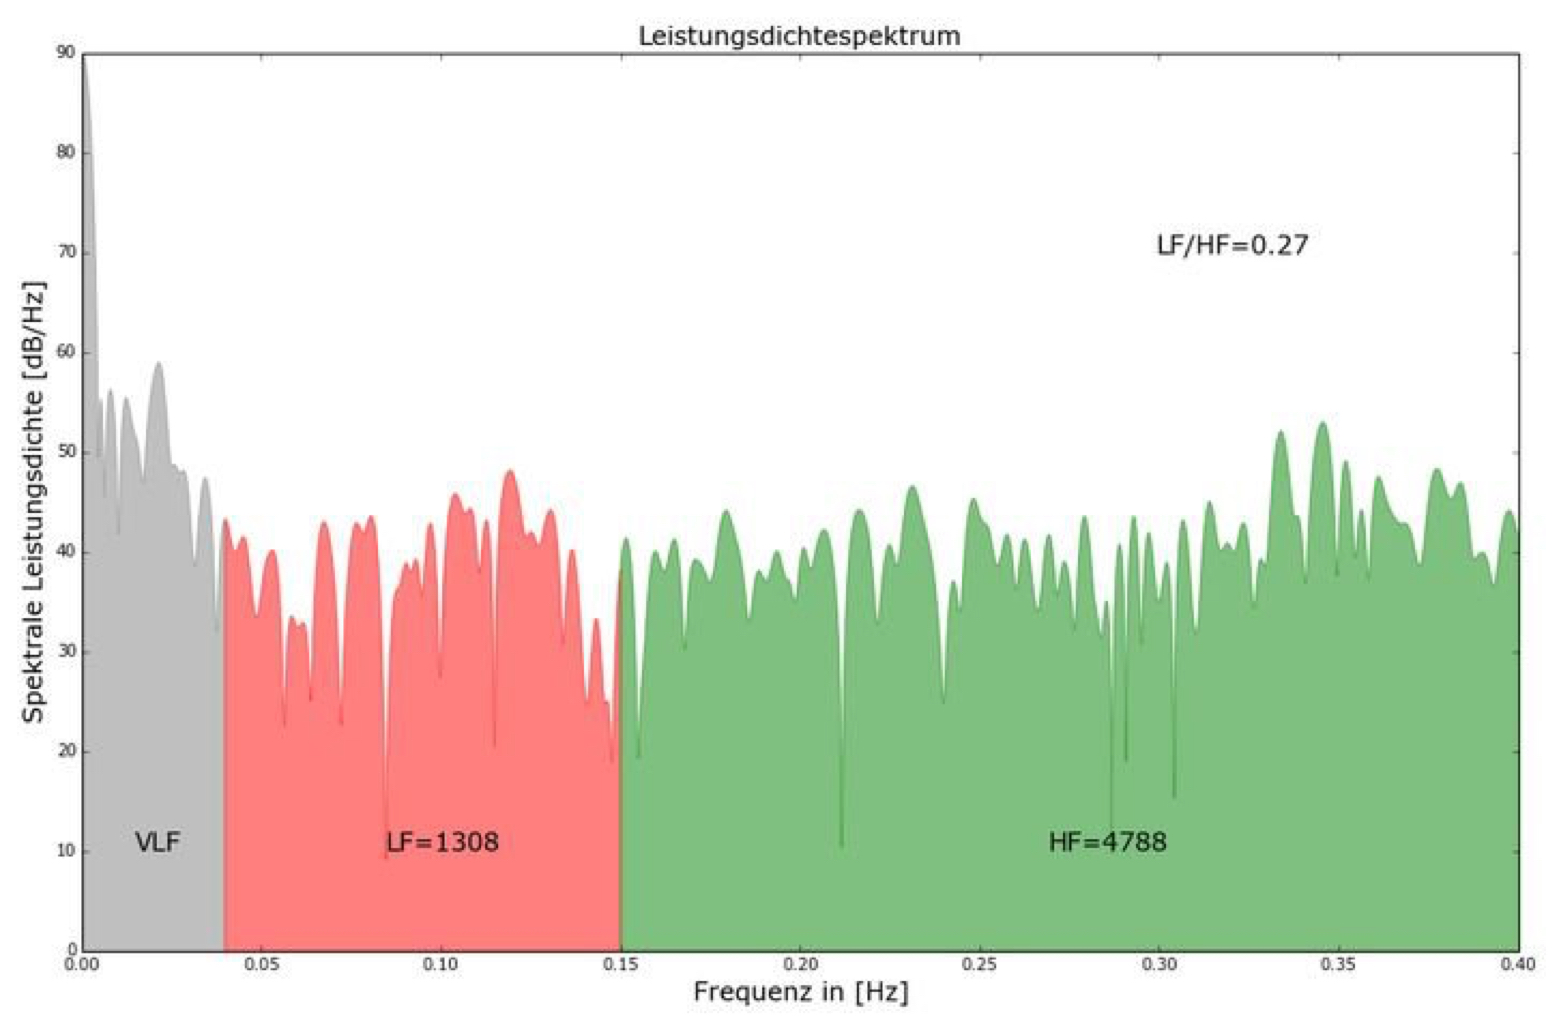
\includegraphics[width=0.9\linewidth]{spec}
 	\caption{Leistungsdichtespektrum}
 	\label{fig:spec}
 	\cite{freque}
 \end{figure}

 
 In \ref{fig:spec} kann die Einteilung der verschiedenen Frequenzbänder gut erkannt werden. Die Messung, welche dem Spektrum zugrunde liegt, ist ein 10-minütige Messung in Ruhe \cite{freque}. Aufgrund dieser kurzen Messdauer ist im Schaubild kein ULF eingetragen. \\
 
 Mithilfe dieser Bereiche können nun folgende frequenzabhängigen Parameter der HRV berechnet werden. 
 \begin{figure}[H]
 	\centering
 	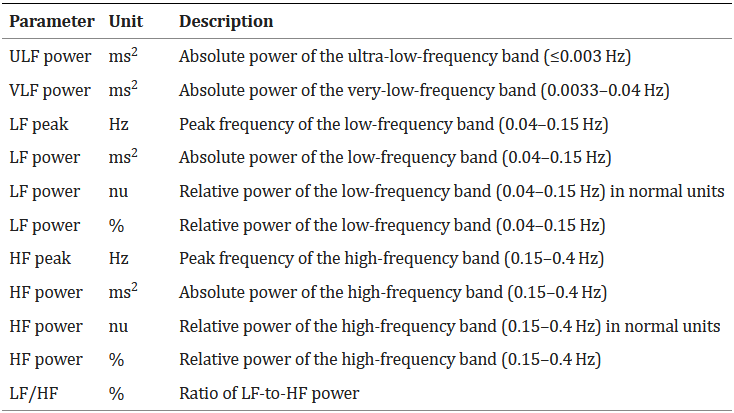
\includegraphics[width=1.0\linewidth]{freqlist}
 	\caption{HRV - Frequenzabhängige Parameter}
 	\label{fig:freqpic}
 	\cite[S.2]{med}
 \end{figure}
 Nun werden einige wichtige frequenzabhängige Parameter genauer untersucht.
 
 \paragraph{HF power}\mbox{} \\
 Der Parameter HF power kann berechnet werde, in dem die Fläche des HF Bands bestimmt wird. Anschaulich kann dies als grün gefärbte Fläche in Abbildung \ref{fig:spec} betrachtet werden. Als Einheit trägt HF power meist ms$^{2}$, kann jedoch auch in Prozent angegeben werden. 
 Mit dem Parameter HF power können parasympathische Aktivitäten gemessen werden, wodurch er im autonomen Nervensystem dem Parasympathikus zugeordnet ist. Aufgrund dieser Tatsache steht er in einem starken Zusammenhang mit RMMSD und pNN 50, welche ebenfalls die Aktivität des Parasympathikus messen. \\
 VLF- und LF power können analog dazu berechnet werden, indem die Fläche im jeweiligen Intervall bestimmt wird. Der Parameter VLF power kann beispielsweise gentzt werden, um Aussagen über SADS (Sudden arrhythmic death syndrome, deutsch: Plötzliche Arrhythmiesyndrome) zu treffen. Auch ist ein niedriger VLF power Wert ein Anzeichen für PTSD (Post Traumatic Stress Disorder, deutsch: posttraumatische Belastungsstörung) . \cite[S.5]{med}
 
 \paragraph{LF/HF}\mbox{} \\
 Ein weiterer Parameter ist das Verhältnis zwischen den Werten von LF und HF. Da LF power eher vom Sympathikus getrieben wird und HF power stark vom Parasympathikus abhängt, kann das Verhältnis aus beiden Werten als Parameter für das Zusammenspiel und die Balance zwischen Sympathikus und Parasympathikus gesehen werden. Ein hoher LF/HF Wert spricht daher eher für eine Dominanz des Sympathikus, während ein geringer Wert des LF/HF Verhältnisses für eine höhere parasympathische Aktivität spricht. \cite[S.5]{med} 
 
 \subsection{Nicht-lineare Parameter}
 
 Die letzte Gruppe der HRV nennt sich \textit{nicht-lineare Parameter} und ist "moderner" als zeitabhängig- oder frequenzabhängige- Parameter. Dies soll bedeutet, dass sie noch nicht so lange existieren als die bereits erläuterten Gruppen. Nichtsdestotrotz sind sie ein wichtiger Teil der Erhebung von HRV Daten und gewinnen immer mehr an Aufmerksamkeit und Bedeutung.\\
 
 Die Frequenzabhängige Analyse kennzeichnet sich durch das Berechnen des Leistungsdichtespektrums. Aus diesem werden dann alle Parameter bestimmt. Auch bei der zeitabhängigen Analyse gibt es einen eindeutigen Weg wie Parameter bestimmt werden. Bei der nicht-linearen Analyse ist dies nicht so. Es gibt keinen eindeutigen "Rechenweg" für die Analyse und Berechnung der Parameter. \\ 
 Eine  weit verbreitete Möglichkeit ist es, die verschiedenen NN-Intervalle in einem Poincaré-Diagramm darzustellen. Aus diesem können anschließend einige Parameter berechnet werden. Eine ausführliche Liste der nicht-linearen Parameter der HRV ist in Abbildung  \ref{fig:nichtlinear} dargestellt.\cite{poincare}
  \begin{figure}[H]
 	\centering
 	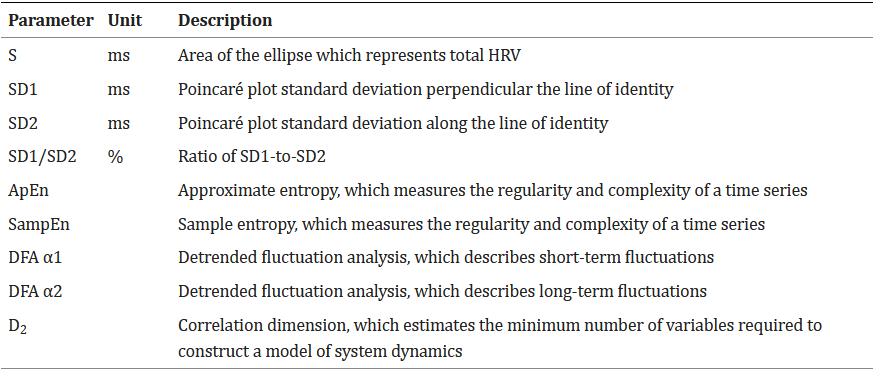
\includegraphics[width=1.0\linewidth]{nichtlinear}
 	\caption{HRV - Nicht-lineare Parameter}
 	\label{fig:nichtlinear}
 	\cite[S.3]{med}
 \end{figure}
 
 Der Poincaré-Plot und die dazugehörige Berechnung der Parameter \textit{SD1} und \textit{SD2} soll im Folgenden genauer betrachtet werden.
 
 \paragraph{Poincaré-Diagramm}\mbox{} \\
 In einem Poincaré-Diagramm werden aufeinanderfolgende NN-Intervalle gegeneinander eingetragen. Dies kann man sich wie folgt vorstellen.
 Der Wert des Intervalls NN$_{n}$  wird als x-Achsenwert eingezeichnet. Das darauffolgende Intervall NN$_{n+1}$ ist der dazugehörige y-Achsen Wert. Dadurch entsteht ein Punkt im Diagramm mit den Koordinaten P(NN$_{n}$ |NN$_{n+1}$). Das nächste Intervall NN$_{n+2}$ ist wieder x-Achsenwert mit dazugehörigem y-Achsenabschnitt bei NN$_{n+3}$. Mithilfe dieser paarweisen Zuordnung werden alle NN-Intervalle der Messung in das Diagramm eingetragen, wodurch eine große Punktewolke entsteht. Ein Beispiel für solch ein  Poincaré-Plot im Kontext der HRV kann in \ref{fig:poincare} gesehen werden. Im Anschluss wird meist eine Ellipse um den Mittelwert gezeichnet. Diese hilft bei der späteren Berechnung der Parameter und kann in Abbildung \ref{fig:SD} gesehen werden.\cite{poincare}

 \begin{figure}[H]
 	\centering
 	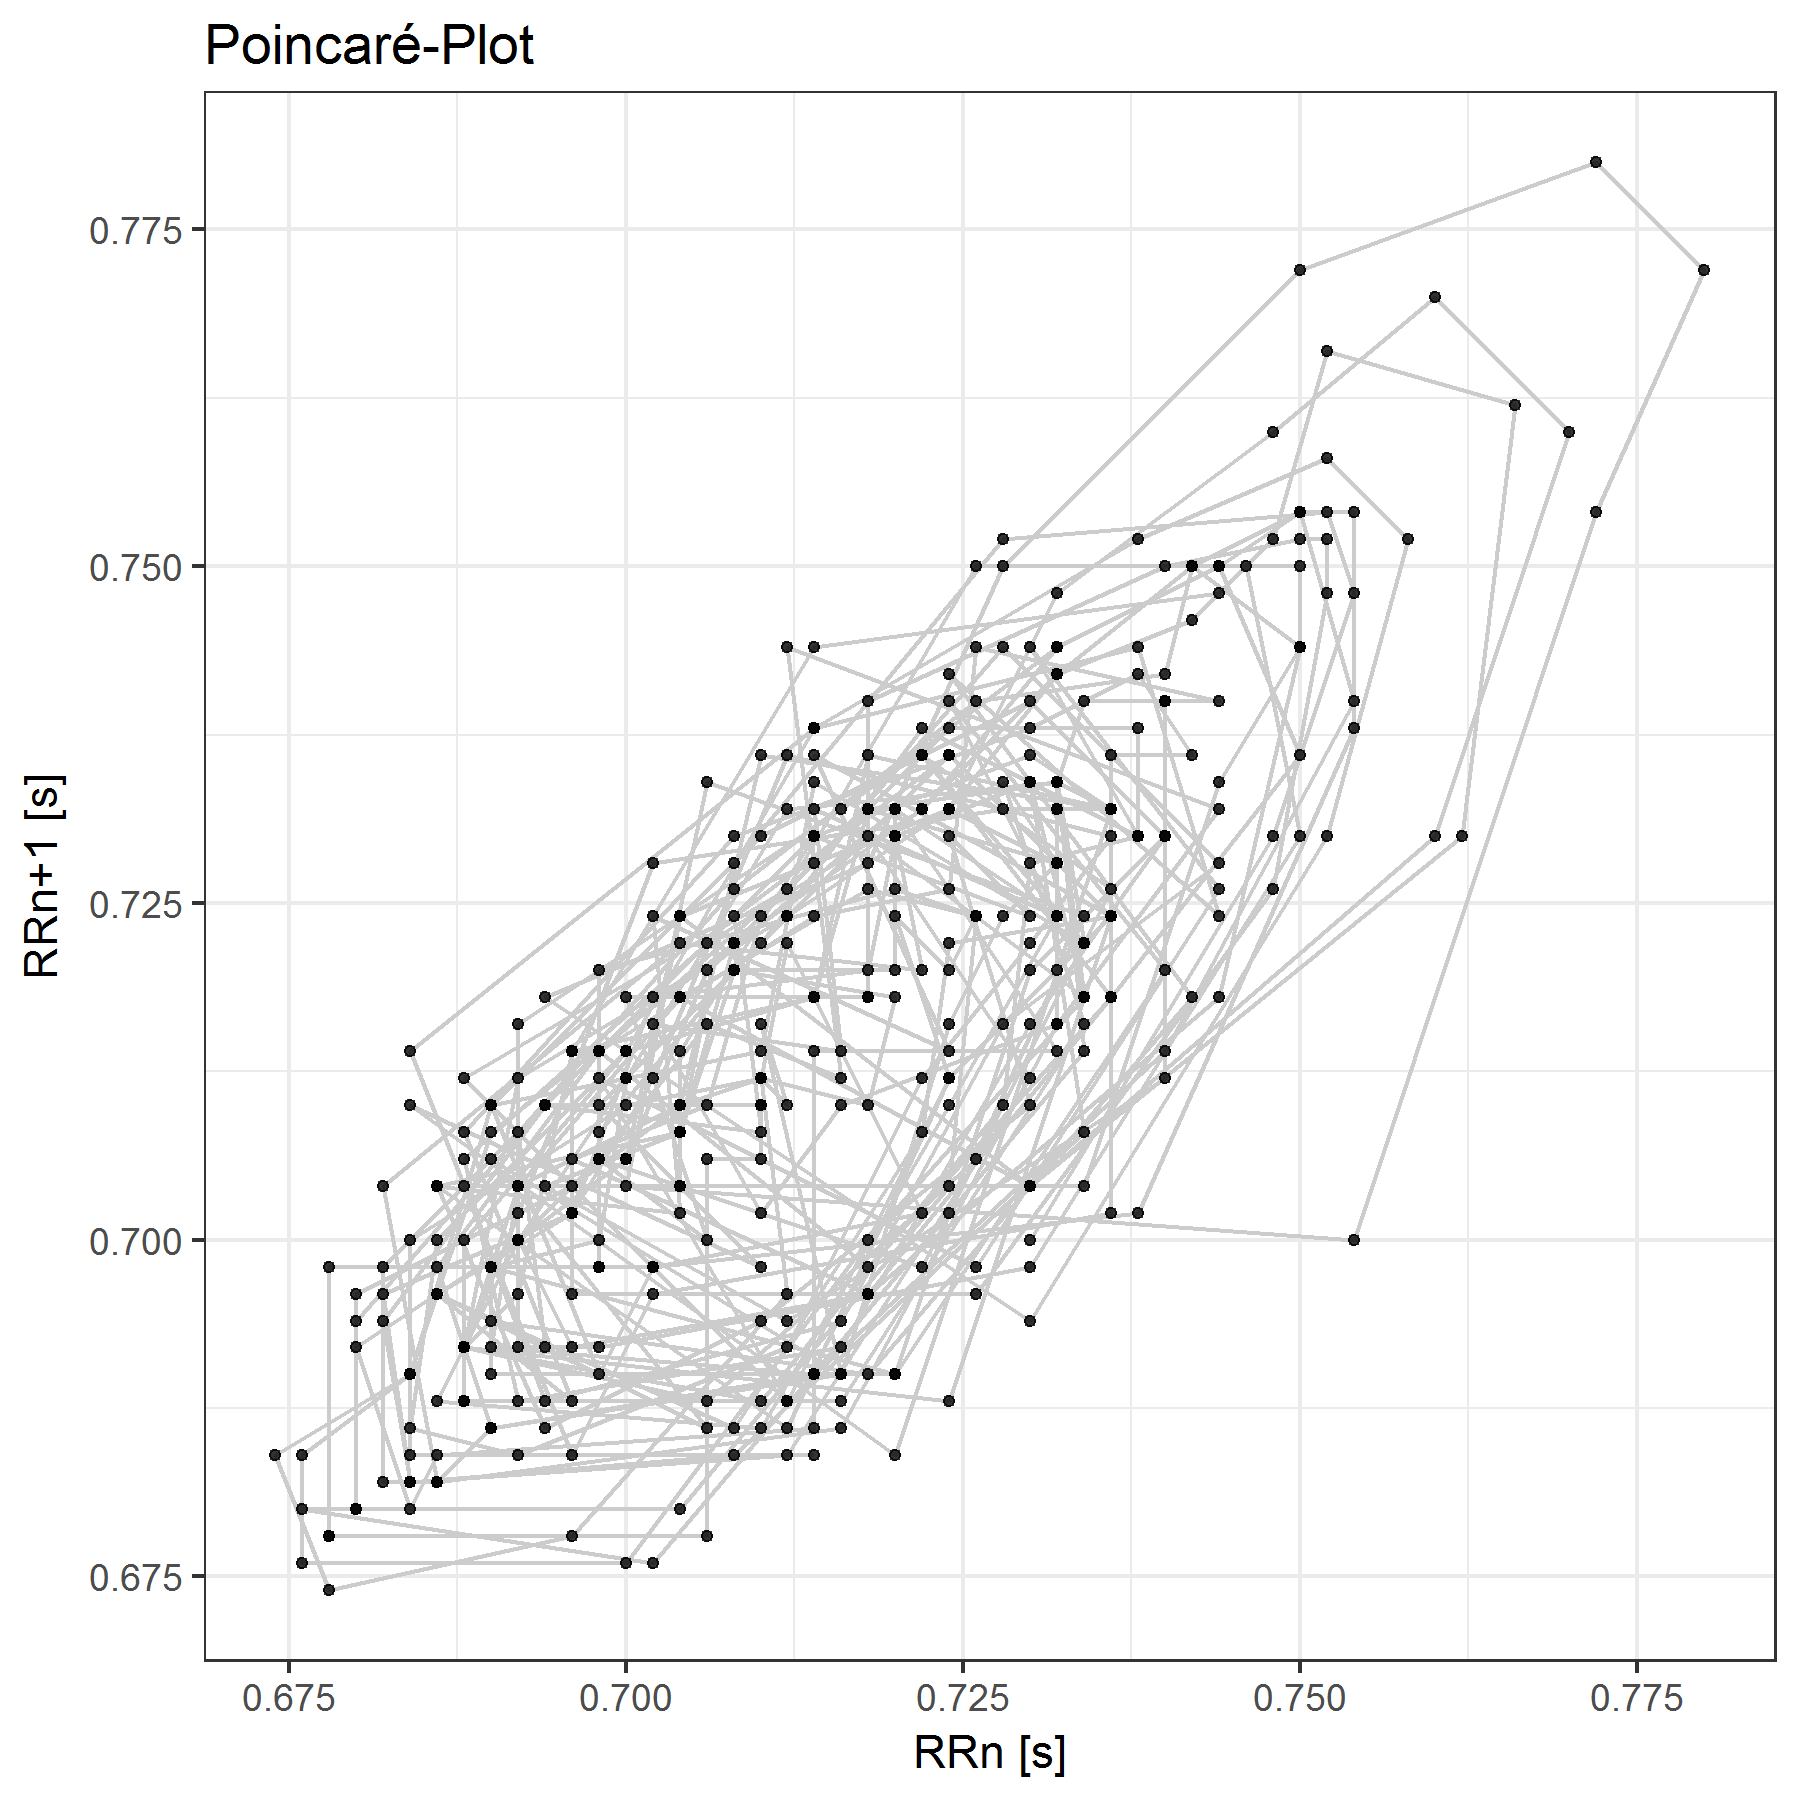
\includegraphics[width=0.7\linewidth]{poincare}
 	\caption{Poincaré-Diagramm}
 	\label{fig:poincare}
 	\cite{poincare}
 \end{figure}

Um mithilfe des Poincaré-Diagramms Aussagen über die Herzratenvariabilität treffen zu können, kann die Form der entstandenen Punktewolke visuell analysiert werden. Bei einer geringen Variabilität des Herzens liegen die Punkte alle nah beisammen und die Punktewolke ist klein. Bei Menschen mit einer hohen HRV ist die ellipsenförmige Punktewolke größer. Auffällige Intervalle, welche auf Messfehler oder Herzfehler zurückzuführen sind, werden im Poincaré-Diagramm als Ausreißer dargestellt. Diese sind weit von der Punktewolke entfernt. In Abbildung \ref{fig:poincare} können einige dieser Ausreißer im oberen rechten Teil erkannt werden.

 \paragraph{SD1 und SD2}\mbox{} \\
 Die bekanntesten Parameter der nicht-linearen Analyse sind SD1 und SD2. Beide dieser Parameter beziehen sich auf die Streuung der Punkte um den Mittelpunkt im Poincaré-Diagramm. Mathematisch betrachtet ist dies die Standardabweichung.\cite{poincare}
 \begin{figure}[H]
	\centering
	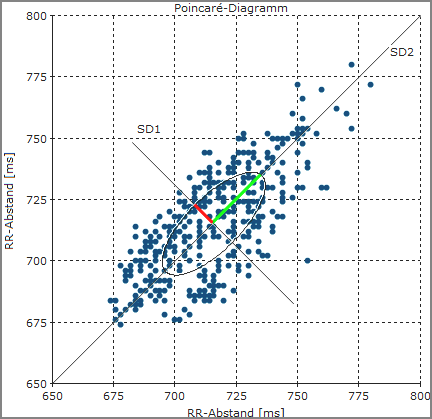
\includegraphics[width=0.6\linewidth]{SD}
	\caption{SD1 und SD2}
	\label{fig:SD}
	\cite{poincare}
\end{figure}

Zur Berechnung des SD1 wird die Standardabweichung in Richtung der linken Diagonalen gemessen. Der Parameter SD1 gibt Hinweise zur Kurzzeitvariabilität. Er ist identisch zum zeitabhängigen Parameter RMSSD \cite[S.6]{med}. \\

Der Parameter SD2 wird durch die Bestimmung der Standardabweichung in der rechen Diagonalen bestimmt. Er drückt eher die Langzeitvariabilität des Herzens aus, sodass er in einem Zusammenhang mit dem frequenzabhängigen Parameter LF power steht. Das Verhältnis der beiden Parameter SD1/SD2 ist ähnlich wie das bereits erläuterte Verhältnis HF/LF. \cite[S.7]{med} 

\subsection{Zusammenfassung}

In diesem Kapitel wurden die verschiedenen Analysen und Parameter der HRV erläutert. Es werden immer neue Parameter entdeckt, welche berechnet werden können. Auffallend ist dabei, dass viele Parameter zusammenhängen. Beispielsweise sind RMSSD und SD1 der gleiche Wert, obwohl diese auf völlig verschieden Arten berechnet werden. Dies zeigt, dass es nicht die einige richtige Analyse gibt, sondern alle ihre Berechtigung haben. Welche Analyse wann eingesetzt wird, hängt hauptsächlich mit der persönlichen Präferenz zusammen.\\
Zusätzlich lässt sich durch das Verwenden verschiedener Analysen die Aussagekraft des Ergebnisses verstärken. Wenn beispielsweise eine Aussage über die parasympathische Aktivität getroffen werden soll, ist das Ergebnis belastbarer, wenn RMSSD, HF power und SD1 berechnet wird, als wenn nur ein Parameter angeführt wird. \\

Die Berechnung aller Parameter per Hand vorzunehmen, würde extrem viel Zeit in Anspruch nehmen. Daher gibt es bereits Programme und Anwendungen, die diese Berechnung der gewünschten Parameter übernehmen. Außerdem ist die Vergleichbarkeit und Verlässlichkeit der aus den Auswertungen resultierenden Ergebnissen größer, wenn diese mit einem öffentlichen Programm durchgeführt werden. Während dieser Arbeit wurde daher ebenfalls ein Programm zur Auswertung verschiedener HRV Messungen benutzt. Die dafür  Anwendung heißt \textit{Kubios HRV Premium} und soll im Nachfolgenden kurz erläutert werden. 

\section{Kubios HRV Premium}
Das während dieser Arbeit verwendete Programm \textit{Kubios HRV Premium} ist eine kostenpflichtige Anwendung des gleichnamigen finnischen Unternehmens Kubios. Wie der Name des Programms bereits sagt, ist dies ein Tool zur Auswertung von Herzratenvariabilität. Dabei können verschiedene Parameter der HRV berechnet und angezeigt werden.
Im Folgenden wird die Anwendung Kubios HRV Premium nur mit dem Namen Kubios angesprochen. 
 \begin{figure}[H]
	\centering
	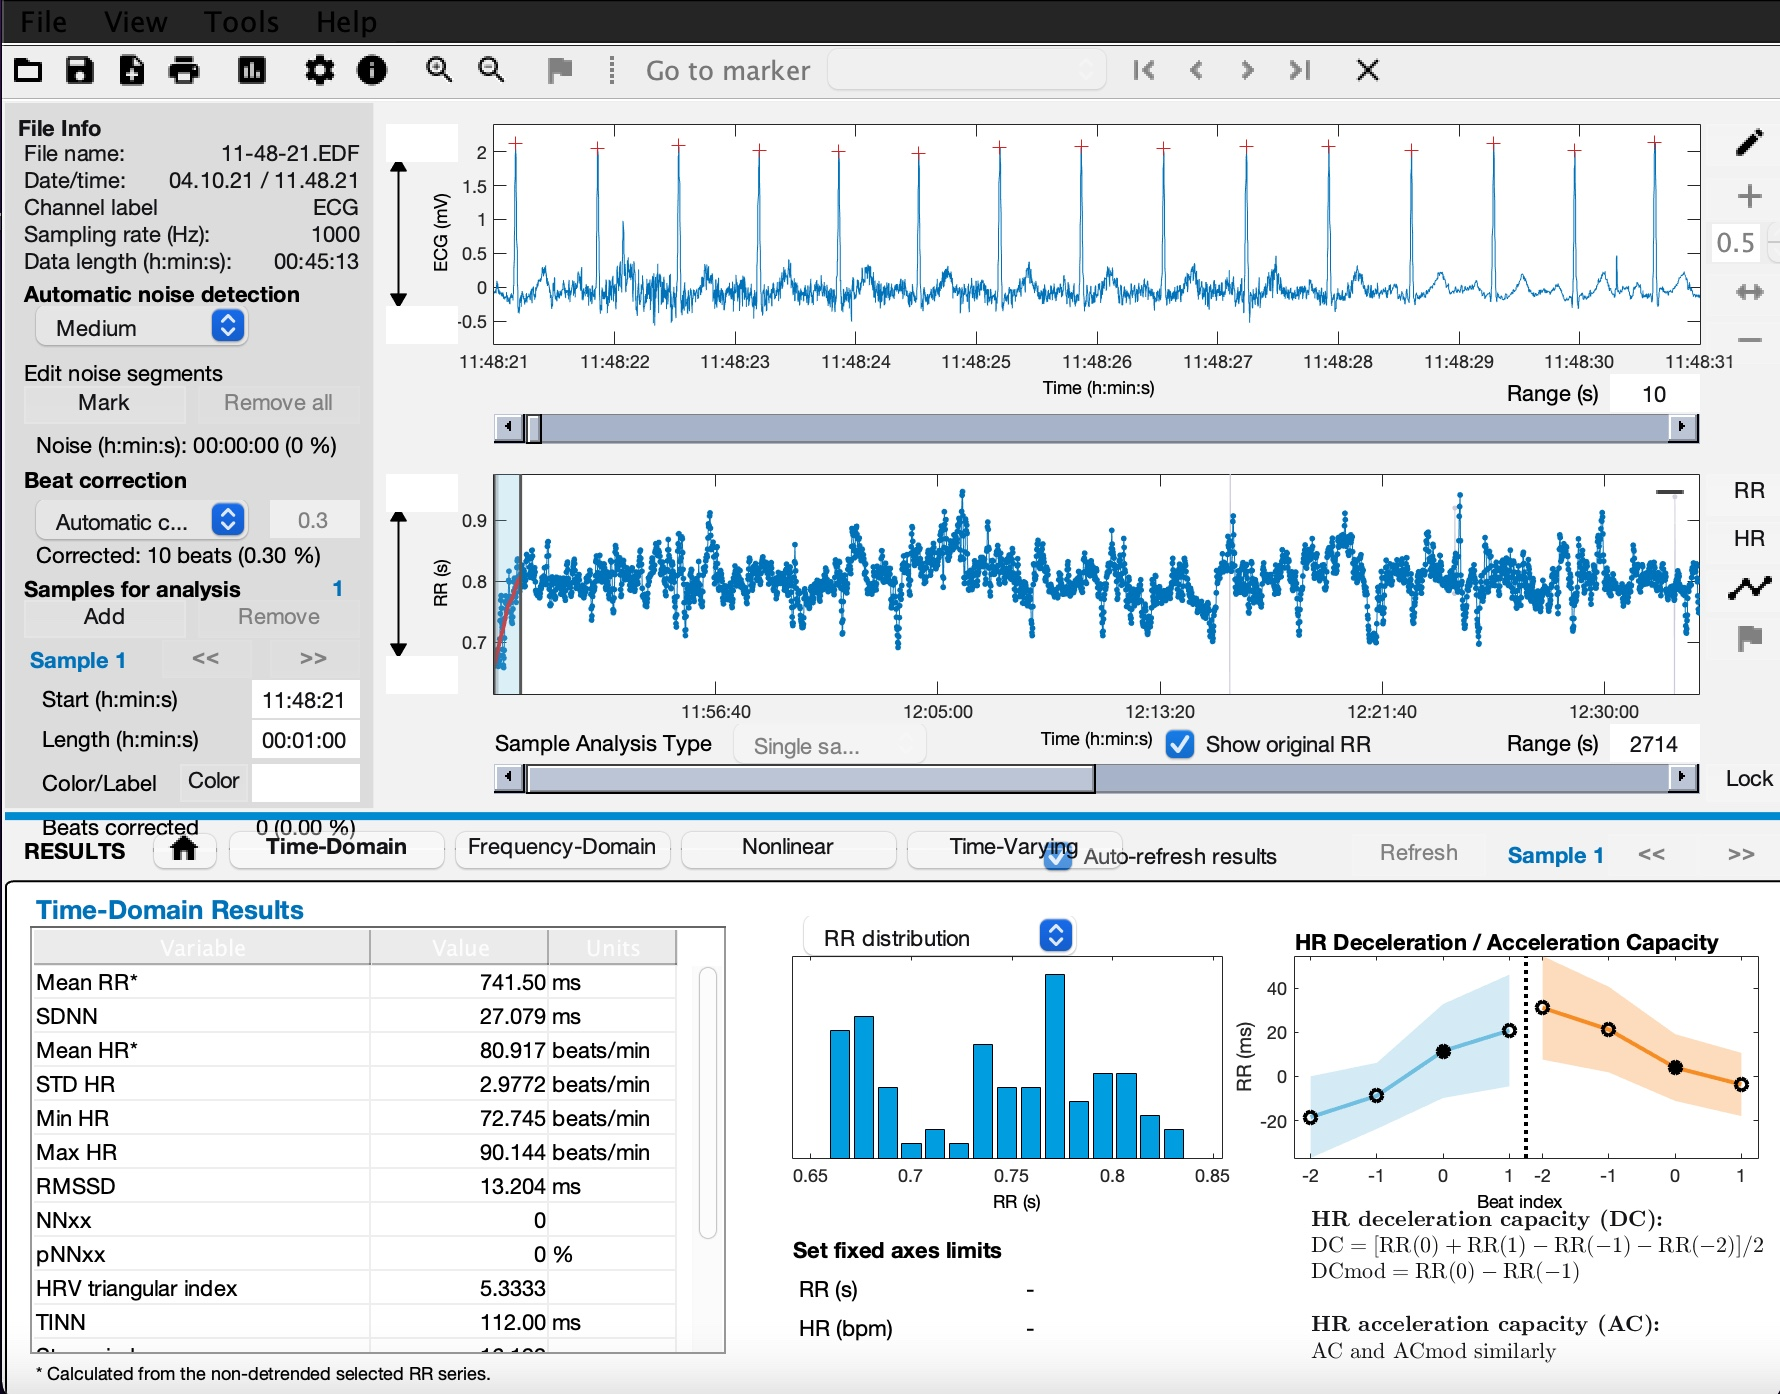
\includegraphics[width=1.0\linewidth]{kubios}
	\caption{Kubios HRV Premium}
	\label{fig:kubios}
\end{figure}

In der gestarteten Anwendung (siehe Abbildung \ref{fig:kubios}) wird oben die Messung dargestellt. Gut erkennbar sind dabei die hohen R-Zacken, welche zum Berechnen der Intervalle benötigt werden. Darunter kann ein weiteres Diagramm erkannt werden. Dies zeigt die bereits berechneten aufeinanderfolgenden RR-Intervalle an. In der unteren Hälfte der Anwendung findet die Auswertung der Messdaten statt. So kann in einem Menü ausgewählt werden, welche Parameter berechnet werden sollen. Dabei kann zwischen den bereits beschriebenen zeitabhängigen-, frequenzabhängigen- oder nicht-linearen-Parametern unterschieden werden. In Abbildung \ref{fig:kubios} sind die zeitabhängigen Parameter ausgewählt, welche unten links aufgelistet sind. Unter anderem können dabei die bereits bekannten Parameter RMSSD und SDNN erkannt werden. Daneben sind weitere Diagramme zur Analyse der HRV, welche für diese Arbeit irrelevant sind und daher nicht weiter ausgeführt werden. Auf eine weitere Funktion von Kubios soll nun genauer eingegangen werden. Das Erstellen von Samples. \\

\subsection{Samples}
Um eine Messung auswerten zu können, kann jedes RR-Intervall als ein Wert betrachtet werden. Eine weitere, übersichtlichere Möglichkeit ist es, aus mehreren Werten das arithmetische Mittel zu bilden, und diesen anschließend als einen Wert zu betrachten. Beispielhaft wird die Berechnung von Samples auf eine Messung mit 6 Messwertens in Abbildung \ref{fig:samples} dargestellt. Die Samplegröße beträgt dabei 3.
 \begin{figure}[H]
	\centering
	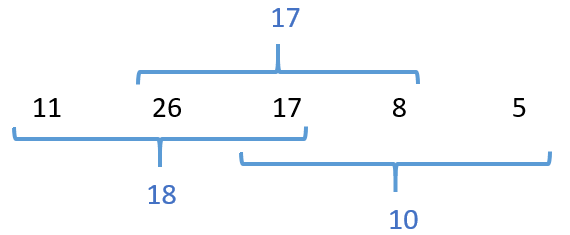
\includegraphics[width=0.6\linewidth]{samples}
	\caption{Berechnung eines Samples}
	\label{fig:samples}
\end{figure}
Aus den Messdaten werden nun Samples berechnet. Der Wert des ersten Samples ergibt sich aus dem arithmetischen Mittel der ersten 3 Werte, was in diesem Fall 18 ergibt. Um nun das zweite Sample berechnen zu können, muss bekannt sein, wie groß der Abstand zwischen den einzelnen Samples ist. In diesem Fall wird jedes Sample immer einen Wert weitergeschoben, wodurch die Werte 26,17 und 8 zur Berechnung des zweiten Samples genutzt werden. Das letzte Sample berechnet sich aus den Werten 17,8 und 5.\\

Die Verwendung von Samples ist auch in Kubios möglich. Dabei muss für jedes Sample  die Größe angegeben werden. In Abbildung \ref{fig:kubiossamples} ist ein Sample der Größe 10 Minuten erstellt worden. Dies bedeutet, dass alle Messwerte dieser 10 Minuten zusammengefasst werden. Für die 40 minütige Messung in Abbildung \ref{fig:kubiossamples} wurde jede Minute ein Sample mit 10 minütiger Länge gestartet.\\

 \begin{figure}[H]
	\centering
	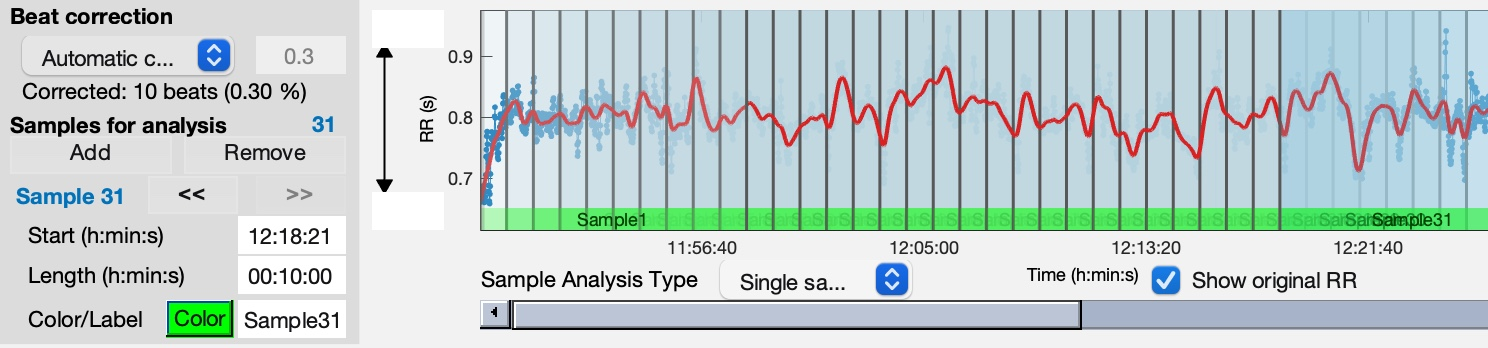
\includegraphics[width=1.0\linewidth]{kubiossamples}
	\caption{Samples in Kubios}
	\label{fig:kubiossamples}
\end{figure}

In Kubios ist es nicht möglich automatisch mehrere Samples anzulegen, weshalb jedes Sample einzeln mit Startzeit und Dauer erstellt werden muss. Für längere Messungen, welche die Erstellung vieler Samples mit sich zieht ist dies daher ein großer Zeitaufwand. Allein für die beispielhafte Messung in Abbildung \ref{fig:kubiossamples} von 40 Minuten ist bei einer Samplegröße von 5 Minuten die manuelle Erstellung von 31 Samples nötig. Eine Automatisierung würde hier viel Zeit und Arbeit sparen. Daher war das automatische Erstellen von Samples in Kubios eines der Hauptziele der Studienarbeit. Weitere Ziele und die Motivation der Arbeit werden in den nächsten Abschnitten erläutert.